\setcounter{figure}{0}

\section{23rd April 2023: The judgment of the Word of God}
\subsection*{Text: Revelation 19:11-21}
  \begin{quote}
    [11] Then I saw heaven opened, and behold, a white horse!  The one
    sitting on it is called Faithful and True, and in righteousness he judges
    and makes war.  [12] His eyes are like a flame of fire, and on his head
    are many diadems, and he has a name written that no one knows but
    himself.  [13] He is clothed in a robe dipped in blood, and the name by
    which he is called is The Word of God.  [14] And the armies of heaven,
    arrayed in fine linen, white and pure, were following him on white
    horses.  [15] From his mouth comes a sharp sword with which to strike
    down the nations, and he will rule them with a rod of iron.  He will
    tread the winepress of the fury of the wrath of God the Almighty.  [16]
    On his robe and on his thigh he has a name written, King of kings and
    Lord of lords.

    [17] Then I saw an angel standing in the sun, and with a loud voice he
    called to all the birds that fly directly overhead, “Come, gather for the
    great supper of God, [18] to eat the flesh of kings, the flesh of
    captains, the flesh of mighty men, the flesh of horses and their riders,
    and the flesh of all men, both free and slave, both small and great.”
    [19] And I saw the beast and the kings of the earth with their armies
    gathered to make war against him who was sitting on the horse and against
    his army.  [20] And the beast was captured, and with it the false prophet
    who in its presence had done the signs by which he deceived those who had
    received the mark of the beast and those who worshiped its image.  These
    two were thrown alive into the lake of fire that burns with sulfur.  [21]
    And the rest were slain by the sword that came from the mouth of him who
    was sitting on the horse, and all the birds were gorged with their flesh.
  \end{quote}
\subsection*{Notes}
\begin{itemize}
  \item{Satan uses false words to lead mankind down the path of destruction.
  Our passage today describes a metaphorical war that takes place after the
  fall of Babylon.  The two bellingerants are the forces of evil (lead by
  Satan, personified by the beast and the false prophet) and the forces of
  good, led by Jesus.}
  \item{In our world today, the beast represents all the human systems and
  powers and institutions that is arrogant and haughty in men that set
  themselves against God.  The false prophets are the spokesmen for these
  human systems and powers and institutions by spreading false messages and
  lies.  One example of such a lie is that we must enjoy our life on earth,
  because ``you only have one life''.  This hedonistic, individualistic lie
  promoted by our culture helps to serve the system of capitalism.  On the
  other hand, in 1 John we see that ``all that is in the world, the desires
  of the flesh and the desire of the eys and the pride of life, is not from
  the Father''.  We also see in Paul that ``Godliness with contentment is
  great gain''.  The lies spoken by the false prophets in the world lead us
  away from God and sometimes set us in opposition to God, which is what
  Satan wants to do!  }
  \item{So as Paul explains, we do not wrestle against flesh and blood, but
  we wrestle against these false ideologies that Satan's false prophets
  spread and we need to wrestle against Satan.  This is our war to fight, as
  Christians.  We do not take up any actual weapons of war.  And as
  Christians in this war, we are led by our Lord Jesus.}
  \item{Our Lord Jesus here in this chapter is described by a rider on a
  white horse, and is called Faithful and True.  Our Lord Jesus here has many
  diadems on his head, and on his robe and his thigh, he has the inscription
  ``King of kings and Lord of lords''.  All of this tell us that Jesus here
  is sovereign over all.  The beast tries to mimic the sovereignty of Jesus
  here (with 10 crowns), but Jesus is the real sovereign.  Our Lord Jesus
  here is also described with the inscription ``Word of God'', which could be
  a throwback to John 1, but some scholars think a better reference would be
  the apocryphal book Wisdom 4:12-13.  In Wisdom 4:12-13, the context is that
  the Word of God came down from heaven in the last plague on Egypt.  Our
  Lord Jesus here defeats the forces of evil with a sharp sword, which are
  his words (c.f also Hebrews 4).  He defeats the forces of evil himself, his
  army does nothing.  }
  \item{After Jesus defeats the forces of evil, the forces of evil are
  pictured to lie dead on the field.  So all who follow the beast and the
  false prophet are to become the supper of God for the birds.  This is a
  very macabre constrast to the marriage supper of the Lamb for the
  redeeemed.  So for those who are faithful, they will enjoy the marriage
  supper of the Lamb; for those who follow the beast and the false prophet,
  their fate is utter defeat; their bodies will not even be buried but will
  become bird food.  The beast and the false prophet are also then thrown
  into the lake of fire.  For us, one aspect of this is that there will be no
  more false ideologies and false words anymore, all the false ideologies and
  false words will be eradicated.}
  \item{We can have faith that this final battle will end in this way, that
  satan and death will be defeated.  We can have such faith in God's word
  because the Word of God has come down to us in the person of Jesus Christ,
  light from light, true God from true God.  Jesus Christ, the Word of God,
  took on human nature for us, died on the cross for us, and was raised for
  us.  Jesus is the fulfilment of the Law and the Prophets, and He is the
  guarantor that God's words are faithful and true because He himself is
  Faithful and True.  Jesus, the Word of God, who is Faithful and True, also
  reveals to us how faithless and false we are.  Jesus was crucified because
  of the sins of sinful humanity.  Jesus' crucifixion reveal to us how
  traitorous we are (through Judas), how faithless we are (through Peter),
  and just how evil we are (the roman soldiers, chief priests and pharisees,
  etc). }
  \item{(I didn't really catch this part so I'm making things up here) Jesus
  has revealed to us that we are supposed to be bird food.  Yet in His grace,
  he has granted us to have eternal life by faith in Him.  That is also His
  victory, that by His blood, he has ransomed a people for God (c.f
  Revelation 5).  }
  \item{\begin{figure}[H]
    \centering
    % 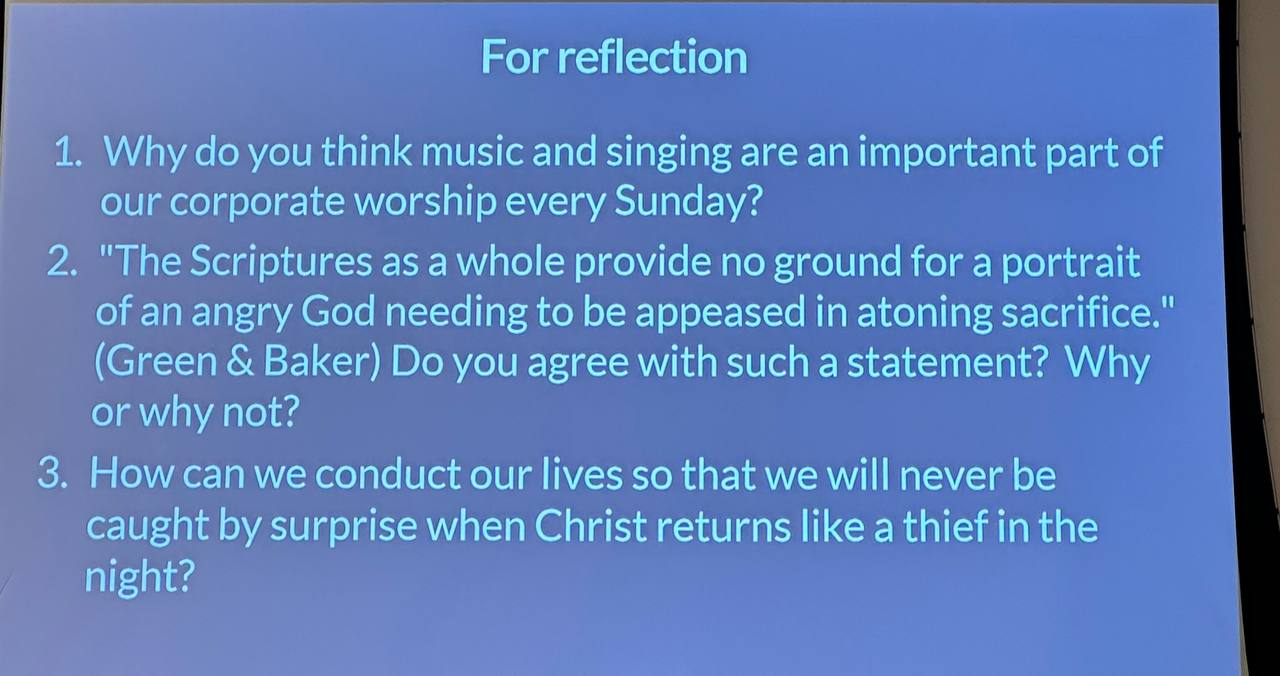
\includegraphics[width=0.8\textwidth, trim={0cm 0cm 0cm 0cm},clip]{Figures/marSermon4Reflections.jpg}
    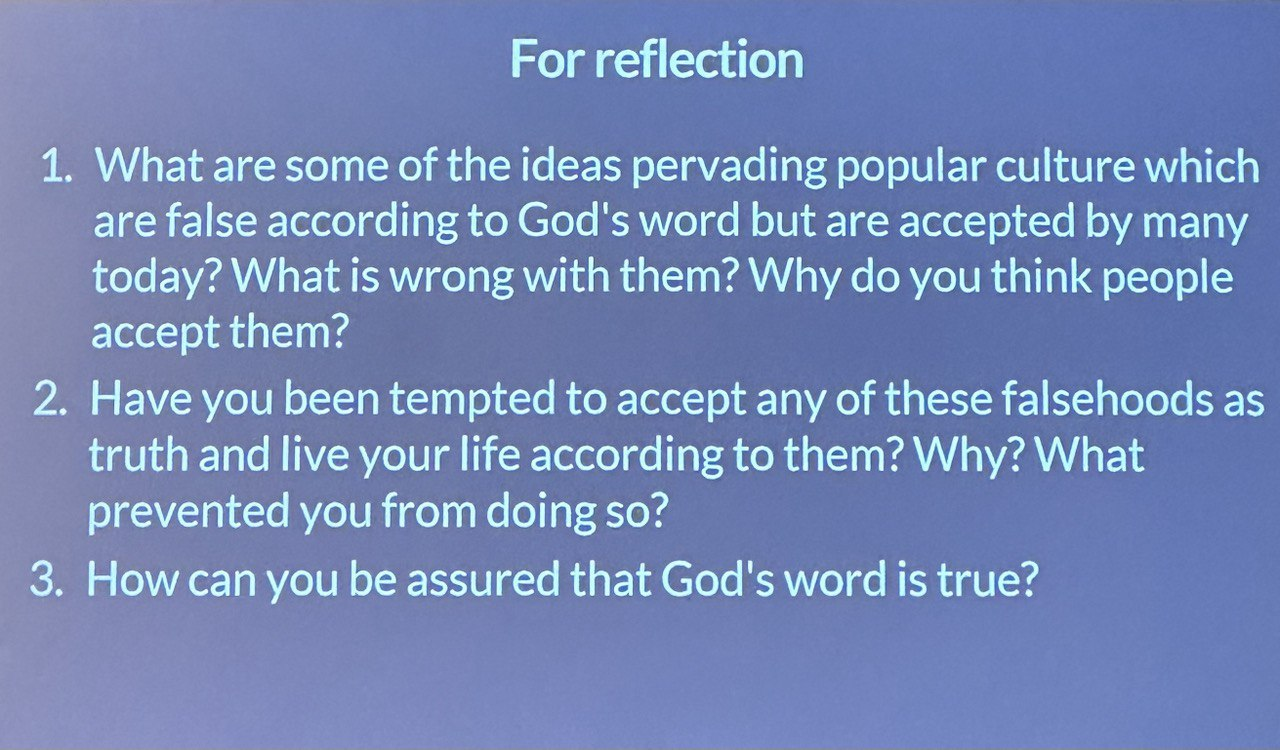
\includegraphics[width=0.8\textwidth, trim={0cm 0cm 0cm 0cm},clip]{Figures/aprilSermon4Reflections.jpg}
    \caption[]{Reflection questions for this sermon}
    \label{}
  \end{figure}}
\end{itemize}